% !TEX root =main.tex
We illustrate our technique on a two-dimensional switched system with $4$ modes. We fix the confidence level, \mbox{$\beta = 0.92$}, and compute the lower and upper bounds on the JSR for $N:=15+15k,\, k \in\{0, \ldots, 23\}$, according to Theorem~\ref{thm:lowerbound} and Theorem~\ref{thm:mainTheorem}, respectively. We illustrate the average performance of our algorithm over $10$ different runs in Fig.~ \ref{fig:11} and Fig.~\ref{fig:21}. Fig.~\ref{fig:11} shows the evolution of $\delta(\beta, N)$ as $N$ increases. We illustrate that $\delta$ converges to $1$ as expected. In Fig.~\ref{fig:21}, we plot the upper bound and lower bound for the JSR of the system computed by Theorem~\ref{thm:mainTheorem} and Theorem~\ref{thm:lowerbound}, respectively. To demonstrate the performance of our technique, we also provide the JSR approximated by the JSR toolbox \cite{jsrtoolbox}, which turns out to be $0.7727$. Note that, the plot for the upper bound starts from $N=45$. This is due to the fact for $N=15$, and $N=30$, $\delta(\beta, \omega_N) = 0$, hence it is not possible to compute a nontrivial upper bound for these small values of $N$. As can be seen, the upper bound approaches to a close vicinity of the real JSR with approximately 200 samples. In addition, the gap between the upper and lower bound converges to a multiplicative factor of $\frac{\rho}{\sqrt{n}}$ as expected.

\begin{figure}
\begin{center}
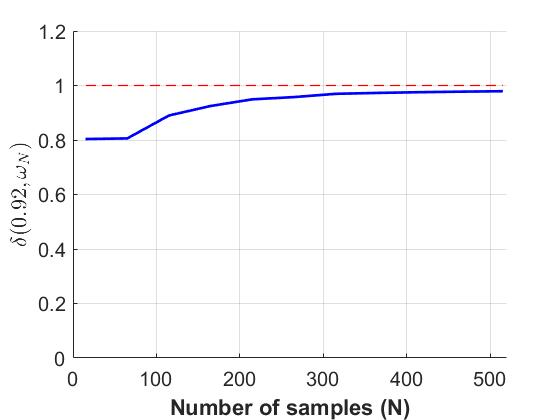
\includegraphics[trim = 5mm 5mm 5mm 5mm, scale=0.35]{delta1.jpg}

\caption{Evolution of $\delta$ with increasing $N$.}
\label{fig:11}
\end{center}
\end{figure}

\begin{figure}
\begin{center}
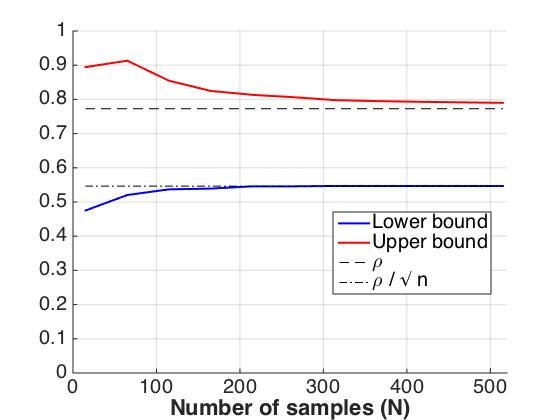
\includegraphics[trim = 5mm 5mm 5mm 5mm,scale=0.35]{bounds1.jpg}

\caption{Evolution of the upper and lower bounds on the JSR with increasing $N$, for $\beta=0.92$.}
\label{fig:21}
\end{center}
\end{figure}

Note that, if we increase the dimension of the switched system, the convergence of $\delta$ to $1$ will become much slower. We confirmed this via experiments up to dimension $n=6$. For example, for dimension $n=4$, it took $N=5,000$ to $N=10,000$ points to reach $\delta = 0.9$. We nevertheless observe convergence of the upper bound to $\rho(\calM)$, and convergence of the lower bound to $\frac{\rho(\calM)}{\sqrt{n}}$. The gap between these two limits is $\frac{\rho}{\sqrt{n}}$ and could be improved by considering a more general class of common Lyapunov functions, such as those that can be described by sum-of-squares polynomials \cite{sosLyap}. We leave this for future work.

Finally, we randomly generate $10,000$ test cases with systems of dimension between $2$ and $7$, number of modes between $2$ and $5$, and size of samples $N$ between $30$ and $800$. We take $\beta = 0.92$ and we check if the upper bound computed by our technique is greater than the actual JSR of the system. We get $9873$ positive tests, out of $10,000$, which gives us a probability of $0.9873$ of the correctness of the upper bound computed. Note that, this probability is significantly above the provided $\beta$. This is expected, since our techniques are based on worst-case analysis and thus fairly conservative.